\section{Examples}
\subsection{Single Linked List}
\begin{lstlisting}[mathescape]
using namespace std;
struct node
{
	int data;
	node *next;
};

class linked_list{
private:
	node *head,*tail;
public:
	linked_list(){
		head = NULL;
		tail = NULL;
	}

	void add_node(int n){
		node *tmp = new node;
		tmp->data = n;
		tmp->next = NULL;

		if(head == NULL){
			head = tmp;
			tail = tmp;
		}
		else{
			tail->next = tmp;
			tail = tail->next;
		}
	}
	
	unsigned int List::sum(){
		unsigned sum = 0;
		for (ListNode* node = first; node != sentinel; node = node->next){
			sum += node->value;
		}
		return sum;
	}
	
	void List::deleteValue(unsigned int value) {
	  if(first != sentinel)
	    {
		  auto it_old = first;
		  if(first->value == value){
			 first = first->next;
			 delete it_old;
		   }
	  else{
  		for(auto it = first->next; it != sentinel; it = it->next )
		  { 
			if(it->next->value == value && it->next != sentinel){
			  it_old = it->next;
			  it->next = it_old->next;
			  delete it_old;
			  break;}
		  }
	   }
	}
}	
};

int main()
{	linked_list a;
	a.add_node(1);
	a.add_node(2);
	return 0;
}
\end{lstlisting}


\section{Double Linked List}
\begin{lstlisting}
struct Node {
	int data;
	struct Node* next; // Ptr to next node
	struct Node* prev; // Ptr to prev node
};
\end{lstlisting}
\begin{center}
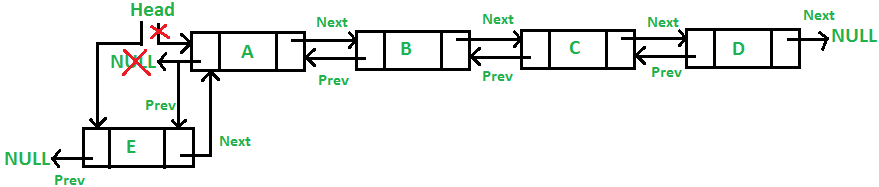
\includegraphics[width=0.24 \textwidth]{images/addFront}
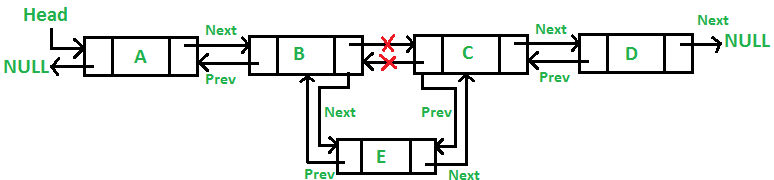
\includegraphics[width=0.24 \textwidth]{images/add_middle}
\end{center}

\begin{lstlisting}
void insertAfter(struct Node* prev_node, int new_data){
	if (prev_node == NULL) {return;}
	struct Node* new_node = (struct Node*)malloc(sizeof(struct Node));
	new_node->data = new_data;
	new_node->next = prev_node->next;
	prev_node->next = new_node;
	new_node->prev = prev_node;
	if (new_node->next != NULL)
		new_node->next->prev = new_node;
}
\end{lstlisting}
\subsection{EBNF}
Diese EBNF definition
\begin{lstlisting}
Hamburger = Bun { Onions } Patties Bun.
Patties = "P" { "P" }.
Onions = "O" "O" "O" { Onions }
Bun = "B"
\end{lstlisting}
Hat folgenden Code als umsetztung mit diesen EBNF inputs als korrekt: "BPB", "BOOOPPB", "BOOOOOOPPPPB"
\begin{lstlisting}
bool Bun(std::istream& is) {
	return consume(is, 'B'); 
	}

// Consumes next Patties = "P" { "P" }.
bool Patties(std::istream& is) {
	if (consume(is, 'P')) {
		while (lookahead(is) == 'P' && consume(is, 'P'));
		return true;
		}
	return false;
}
// Consumes next Onions = "O" "O" "O" { Onions }.
bool Onions(std::istream& is) {
	if (consume(is, 'O')) {
		unsigned int count = 1;
		while (lookahead(is) == 'O' && consume(is, 'O'))
			{++count;}
		return count % 3 == 0; // Zeigt "O" "O" "O" true
		}
	return false;
}
// Consumes next Hamburger = Bun { Onions } Patties Bun.
bool Hamburger(std::istream& is) {
	if (Bun(is)) {
		if (lookahead(is) == 'O' && !Onions(is))
			{return false;}
		if (!(Patties(is) && Bun(is)))
			{return false;}
		return !lookahead(is);
	}
	return false;
}
\end{lstlisting}


\subsection{Klassen \& Operator überschreiben}
Header file mit Klasse
\begin{lstlisting}
class Vec3 {
	public:
	Vec3() 
	: m_x(0.0f), m_y(0.0f), m_z(0.0f) {}
	
	Vec3(float x, float y, float z) 
	: m_x(x), m_y(y), m_z(z) {}
	
	// Access the vector components  
	float x() const { return m_x; }
	float y() const { return m_y; }
	float z() const { return m_z; }
	
	// Set the vector components
	void setX(float x) { m_x = x; }
	void setY(float y) { m_y = y; }
	void setZ(float z) { m_z = z; }
	
	// Compute the norm of vec
	float norm() const;
	// Return a normalized copy of a vector
	Vec3 normalized() const;
	
	// Compute the dot product between the vector and other
	float operator*(const Vec3& other) const;
	
	// Arithmetic operations with vectors
	Vec3& operator+=(const Vec3& other);
	Vec3 operator+(const Vec3& other) const;
	Vec3& operator-=(const Vec3& other);
	Vec3 operator-(const Vec3& other) const;
	
	// Arithmetic operations with scalars
	Vec3& operator/=(float scalar);
	Vec3 operator/(float scalar) const;
	Vec3& operator*=(float scalar);
	Vec3 operator*(float scalar) const;
	
	// Stream operator to display the vector's components
	// "friend" makes sure we can implement it in the class
	friend std::ostream& operator<<(std::ostream& out, const Vec3& v);
	
	// Stream operator to read the vector's components
	// "friend" makes sure we can implement it in the class
	friend std::istream& operator>>(std::istream& in, Vec3& v);
	
	private:
	float m_x;
	float m_y;
	float m_z;
};
\end{lstlisting}
.cpp File
\begin{lstlisting}
float Vec3::norm() const {
	return std::sqrt((*this) * (*this));
}

Vec3 Vec3::normalized() const {
	return (*this) / norm();
}

float Vec3::operator*(const Vec3& other) const {
	return m_x * other.m_x + m_y * other.m_y + m_z * other.m_z;
}

Vec3& Vec3::operator/=(float scalar) {
	m_x /= scalar;
	m_y /= scalar;
	m_z /= scalar;
	return *this;
}

Vec3 Vec3::operator/(float scalar) const {	Vec3 other(m_x, m_y, m_z);
	other /= scalar;
	return other;
}

Vec3& Vec3::operator*=(float scalar) {
	m_x *= scalar;
	m_y *= scalar;
	m_z *= scalar;
	return *this;
}
Vec3 Vec3::operator*(float scalar) const {
	Vec3 other(m_x, m_y, m_z);
	other *= scalar;
	return other;
}
std::ostream& operator<<(std::ostream& out, const Vec3& v) {
	return out << "[" << v.x() << ", " << v.y() << ", " << v.z() << "]";
}

std::istream& operator>>(std::istream& in, Vec3& v) {
	float x, y, z;
	char split;
	in >> std::ws;
	in >> x;
	in >> std::ws;
	in >> split;
	in >> std::ws;
	assert(split == ',');
	in >> y;
	in >> std::ws;
	in >> split;
	in >> std::ws;
	assert(split == ',');
	in >> z;
	v.setX(x);
	v.setY(y);
	v.setZ(z);
	return in;
}

Vec3& Vec3::operator+=(const Vec3& other) {
	m_x += other.m_x;
	m_y += other.m_y;
	m_z += other.m_z;
	return *this;
}

Vec3 Vec3::operator+(const Vec3& other) const {
	Vec3 sum(m_x, m_y, m_z); 
	sum += other;
	return sum;
}

Vec3& Vec3::operator-=(const Vec3& other) {
	m_x -= other.m_x;
	m_y -= other.m_y;
	m_z -= other.m_z;
	return *this;
}

Vec3 Vec3::operator-(const Vec3& other) const {
	Vec3 difference(m_x, m_y, m_z);
	difference -= other;
	return difference;
}
\end{lstlisting}
